% This is the code that generates the slides we'll use for this section.
% If you'd simply like to view the slides, please open slides.pdf


\documentclass[10pt, aspectratio=169]{beamer}

\makeatletter
  \def\beamer@calltheme#1#2#3{%
    \def\beamer@themelist{#2}
    \@for\beamer@themename:=\beamer@themelist\do
    {\usepackage[{#1}]{\beamer@themelocation/#3\beamer@themename}}}

  \def\usefolder#1{
    \def\beamer@themelocation{#1}
  }
  \def\beamer@themelocation{}

\usefolder{../__resources__/beamer_theme}
\usetheme{nathan}

\addtobeamertemplate{navigation symbols}{}{%
    \usebeamerfont{footline}%
    \usebeamercolor[fg]{footline}%
    \hfill%
    \insertframenumber/\inserttotalframenumber
}

\title{Computational Decision Making for Regular People}
\subtitle{04: Modeling Techniques}
\date{November 5, 2024}

\usepackage[font=tiny,labelfont=bf]{caption}
\usepackage{caption}
\captionsetup[figure]{labelformat=empty}

\usepackage{listings}
\usepackage{dirtree}

\begin{document}

\begin{frame}
    \maketitle
\end{frame}

\begin{frame}{Today's Outline}
    \begin{columns}
        \begin{column}{0.5\textwidth}
            \begin{enumerate}
                \item Refresher on Math Modeling (Route Planning Problem)
                \item Handling Multiple Sets At Once
                \item Handling Multiple Time Periods (Talk about which set of parameters to use prior or latter)
                \item Example: Multiple Time Periods
                \item Handling Uncertainty
                \item Example: Multiple Scenarios
                \item Linearization
                \begin{itemize}
                    \item Binary Activation ("Big M")
                    \item "If" statements
                    \item "Max" statements
                    \item "Min" statements
                    
                \end{itemize}
            \end{enumerate}
        \end{column}
        \begin{column}{0.5\textwidth}
            \begin{figure}
                \begin{figure}
                    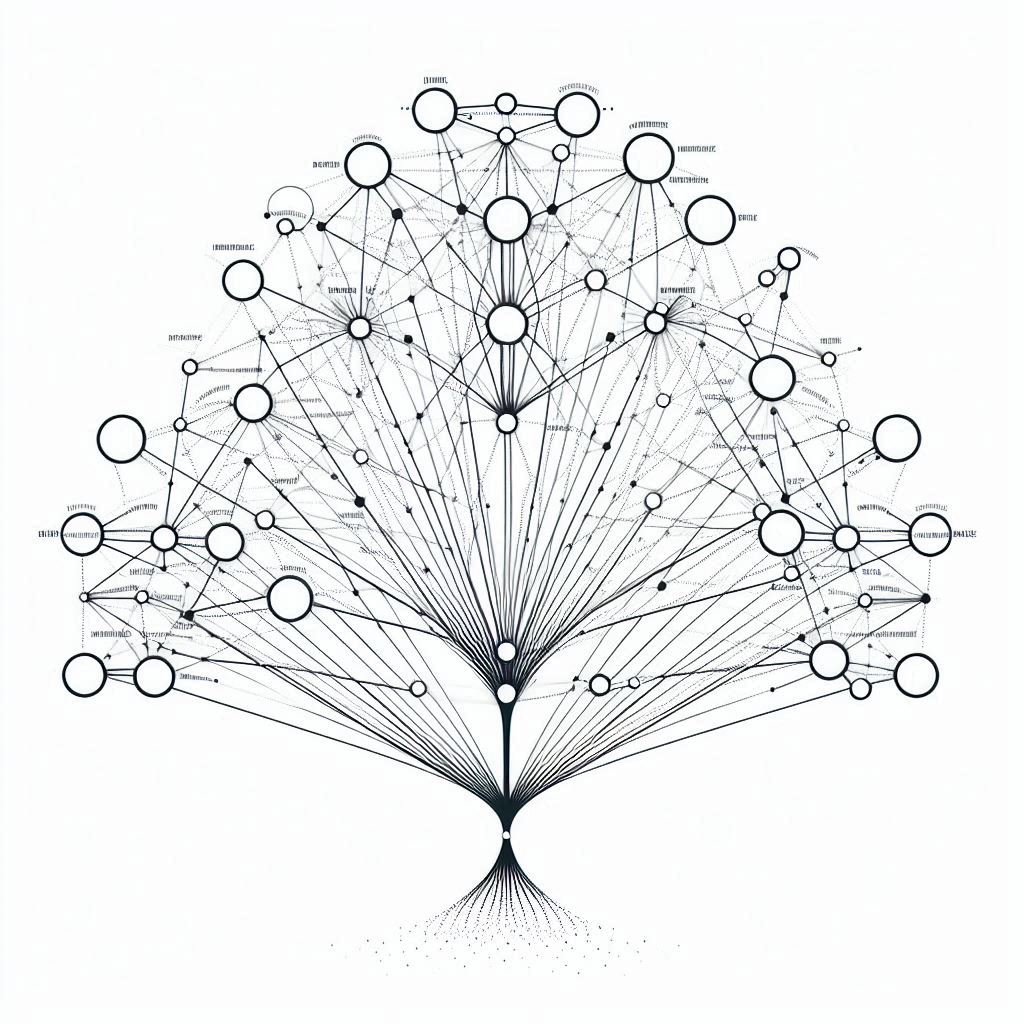
\includegraphics[width=0.95\linewidth]{DecisionTree.png}
                    \caption{This image was created with the assistance of DALL·E 3}
                \end{figure}
            \end{figure}
        \end{column}
    \end{columns}
\end{frame}

\begin{frame}{A Note on Today's Class}
    \begin{center}
        Today we're going to cover a lot of material to set us up for next week when we have to tools to address real-life problems.

        \vspace{1cm}

        We'll cover a variety of individual "tools" that are somewhat disconnected from each other.

        \vspace{1cm}

        If you're feeling lost, that's okay. Go back and reference specific sections of these slides / jupyter notebooks to refresh your mind on how to use each tool if and when you need to use it.
    \end{center}
\end{frame}

\begin{frame}{Refresher on Math Modeling}
    \begin{columns}
        \begin{column}{0.5\textwidth}
            \begin{figure}
                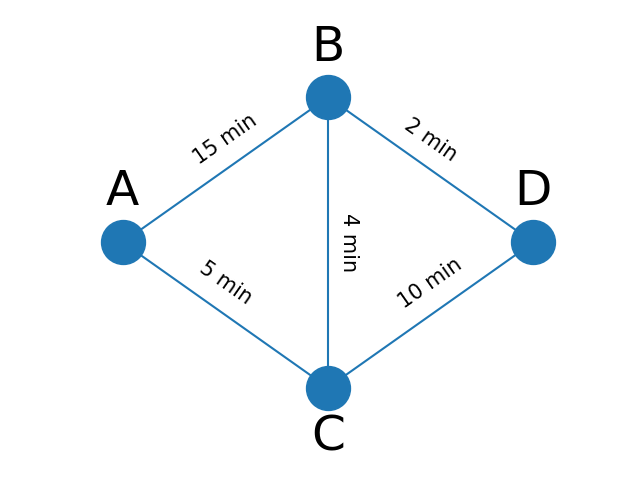
\includegraphics[width=\linewidth]{../01_Introduction/RoutePlanningProblem.png}
            \end{figure}
        \end{column}
        \begin{column}{0.5\textwidth}
            $$---\text{ FULL FORMULATION }---$$
            $$\min_{X_r,Y_p} \sum_{r \in \textbf{R}} \delta_r X_r$$
            $$s.t.\ \ \ \sum_{r \in \textbf{R}_p} X_r = 2 Y_p \ \ \ \forall p \in \textbf{P}^{NON-TERM}$$
            $$\sum_{r \in \textbf{R}_p} X_r = Y_p \ \ \ \forall p \in \textbf{P}^{TERM}$$
            $$Y_p = 1 \ \ \ \forall p \in \textbf{P}^{TERM}$$
            $$X_r, Y_p \in \{0,1\}$$
        \end{column}
    \end{columns}
\end{frame}

\begin{frame}{Handling Multiple Sets}
    \begin{columns}
        \begin{column}{0.5\textwidth}
            \begin{center}
                \textbf{Single Set:}
                $$X_r \ \ \ \forall r \in \textbf{R}$$
                $$Y_p = 1 \ \ \ \forall p \in \textbf{P}^{INIT}$$
            \end{center}
        \end{column}
        \begin{column}{0.5\textwidth}
            \begin{center}
                \textbf{Multiple Sets:}
                $$X_{r,t} \ \ \ \forall r \in \textbf{R}, t \in \textbf{T}$$
                $$Y_{p,t} = 1 \ \ \ \forall p \in \textbf{P}^{INIT}, t \in \textbf{T}$$
            \end{center}
        \end{column}
    \end{columns}
    \vspace{1 cm}
    \begin{itemize}
        \item Index each variable by multiple indices
        \item Iterate constraints and/or definitions over multiple sets
        \item An individual variable, constraint, or definition will be made for \textbf{every combination} of elements between the sets.
        \item In your code, you'll use the multiplication operator ($*$) to create these combinations of sets:
    \end{itemize}

    \begin{tabular}{c c c }
        $\textbf{R} = \{A,B\}$ & $\textbf{T} = \{0,1,2\}$ & $\textbf{R} * \textbf{T} = \{(A,0),(A,1),(A,2),(B,0),(B,1),(B,2)\}$\\
    \end{tabular}
\end{frame}

\begin{frame}{Handling Multiple Time Periods}
    \begin{columns}
        \begin{column}{0.5\textwidth}
            \begin{itemize}
                \item Start by defining a new set ($\textbf{T}$) of each of the time periods you'd like to consider
                \item It's good to fill $\textbf{T}$ with integers so that you can keep track of which time period is before/after which other time period.
                \item For each parameter, variable, and constraint that changes with time, expand it to also iterate over this new time set.
                \item Give special consideration/reformulation to the initial and final time point. \textbf{The constraints for these time points are likely to be different}. ($\textbf{T} \rightarrow \textbf{T}^{NON-TERM}$)
            \end{itemize}
        \end{column}
        \begin{column}{0.5\textwidth}
            \begin{figure}
                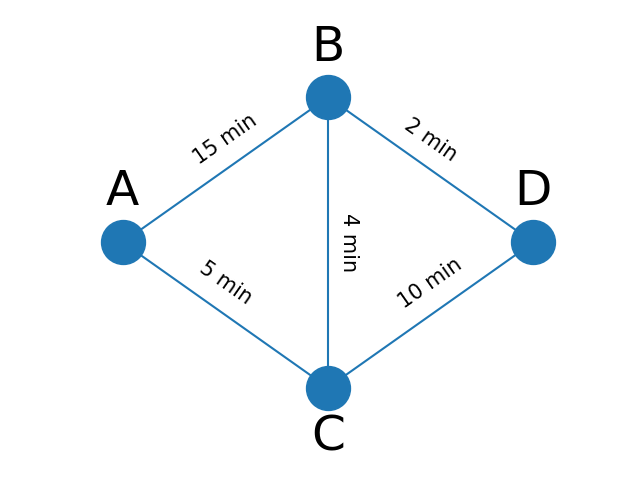
\includegraphics[width=0.6\linewidth]{../01_Introduction/RoutePlanningProblem.png}
            \end{figure}
            \begin{figure}
                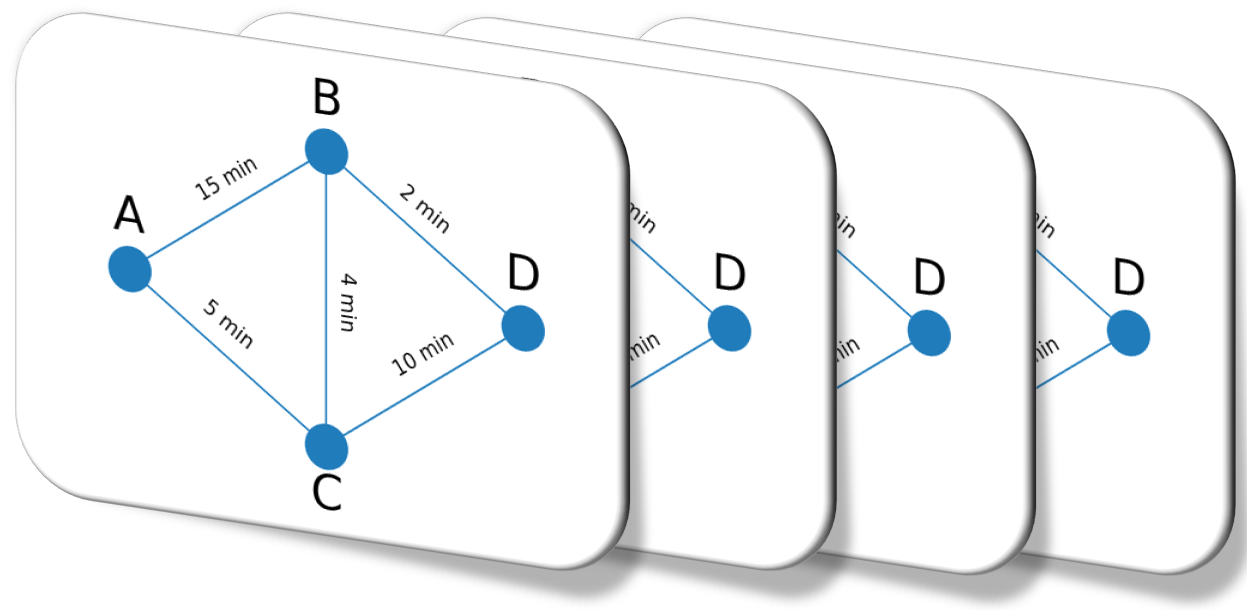
\includegraphics[width=0.7\linewidth]{RoutePlanningProblemRepeated.png}
            \end{figure}
        \end{column}
    \end{columns}
\end{frame}

\begin{frame}{Example: Multiple Time Periods}
    \begin{columns}
        \begin{column}{0.5\textwidth}
            \begin{center}
                \begin{figure}
                    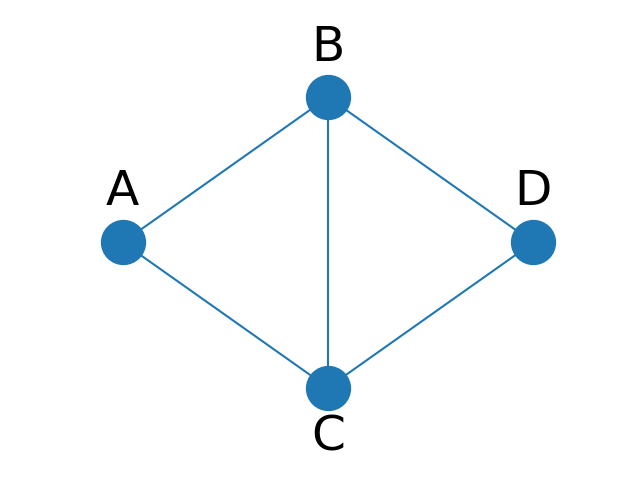
\includegraphics[width=0.6\linewidth]{RoutePlanningProblemBlank.png}
                \end{figure}
                \vspace{-0.2cm}
                To keep things simple, let's assume that instead of time, $\delta_{r,t}$ how represents a toll amount.

                \vspace{0.2cm}

                \begin{tabular}{|c||c|c|c|c|}
                    \hline
                    $r$ & $t=0$ & $t=1$ & $t=2$ & $t=3$ \\
                    \hline \hline
                    $AB$ & \$15 & \$10 & \$8 & \$8\\
                    \hline
                    $AC$ & \$5 & \$5 & \$9 & \$10\\
                    \hline
                    $BC$ & \$4 & \$10 & \$13 & \$13\\
                    \hline
                    $BD$ & \$2 & \$2 & \$6 & \$5\\
                    \hline
                    $CD$ & \$10 & \$15 & \$4 & \$7\\
                    \hline
                \end{tabular}
            \end{center}
        \end{column}
        \begin{column}{0.5\textwidth}
            \begin{center}
                \textbf{Try on your own (on paper or your computer) to come up with how this problem should be re-formulated.}

                \vspace{0.2cm}

                (5 minutes)
            \end{center}
        \end{column}
    \end{columns}
\end{frame}

\begin{frame}{Example: Multiple Time Periods}
    \begin{columns}
        \begin{column}{0.5\textwidth}
            \begin{figure}
                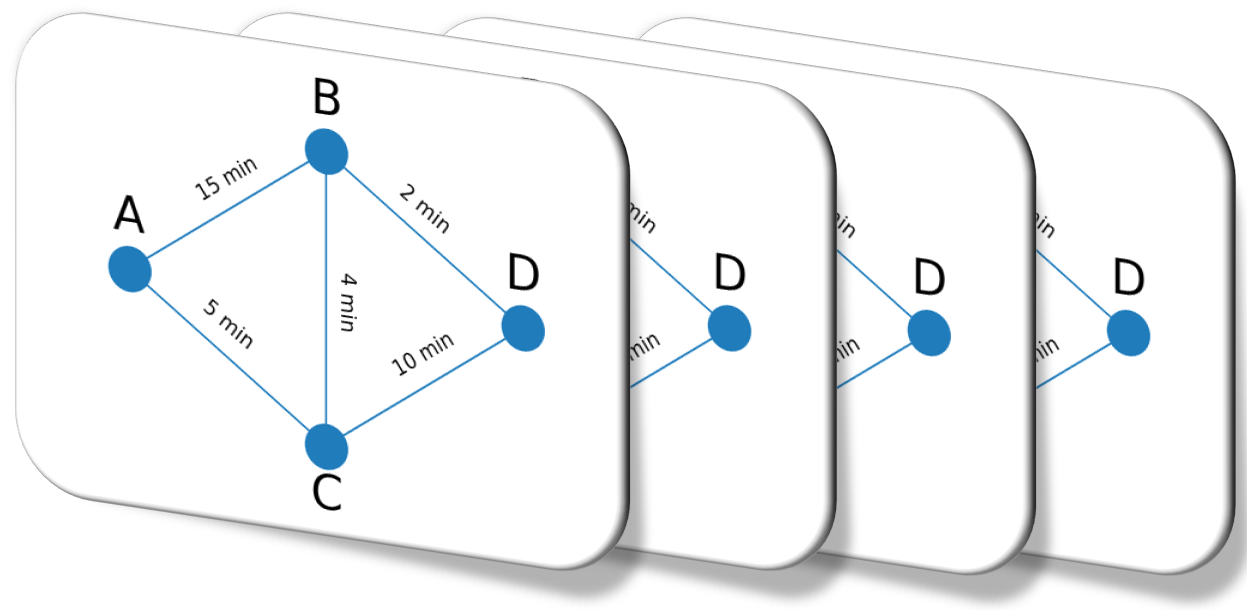
\includegraphics[width=0.7\linewidth]{RoutePlanningProblemRepeated.png}
            \end{figure}
        \end{column}
        \begin{column}{0.5\textwidth}
            $$\min_{X_{r,t},Y_{r,t}} \sum_{r \in \textbf{R}} \sum_{t \in \textbf{T}} \delta_{r,t} X_{r,t}$$
            $$s.t.\ \ \ Y_{p,t+1} - Y_{p,t} = \sum_{r\in\textbf{R}^+_p} X_{r,t} - \sum_{r\in\textbf{R}^-_p} X_{r,t}$$
            $$\phantom\ \ \ \ \ \ \ \ \ \ \ \ \ \ \ \ \ \ \ \ \ \ \ \ \ \ \ \ \ \forall p \in \textbf{P}, t \in \textbf{T} \neq 3$$
            $$\sum_{r \in \textbf{R}} X_{r,t} \leq 1 \ \ \ \forall t \in \textbf{T}$$
            $$\sum_{p \in \textbf{P}} Y_{p,t} = 1 \ \ \ \forall t \in \textbf{T}$$
            $$Y_{A,0} = 1$$
            $$Y_{2,D} = 1$$
            $$X_{r,t}, Y_{p,t} \in \{0,1\}$$
        \end{column}
    \end{columns}
    \begin{center}
        \textit{The code and solution for this problem can be found in the "Solutions.ipynb" notebook in this week's folder.}
    \end{center}
\end{frame}

\begin{frame}{Handling Uncertainty}
    \begin{columns}
        \begin{column}{0.5\textwidth}
            \begin{itemize}
                \item This is an active field of research. If you're interested in learning more, the words to look up are "Stochastic Programming".
                \item Scenarios ($s \in \textbf{S}$)
                \begin{itemize}
                    \item An enumeration of all possible outcomes
                    \item Each path should have an associated probability $\pi_s$
                    \item All probabilities should sum to 1 (100\%)
                \end{itemize}
                \item Coming up with these is one of the hardest parts
                \begin{itemize}
                    \item Virtually impossible to enumerate \textbf{all} outcomes.
                    \item Very hard to estimate the probability of each outcome.
                \end{itemize}
            \end{itemize}
        \end{column}
        \begin{column}{0.5\textwidth}
            \begin{figure}
                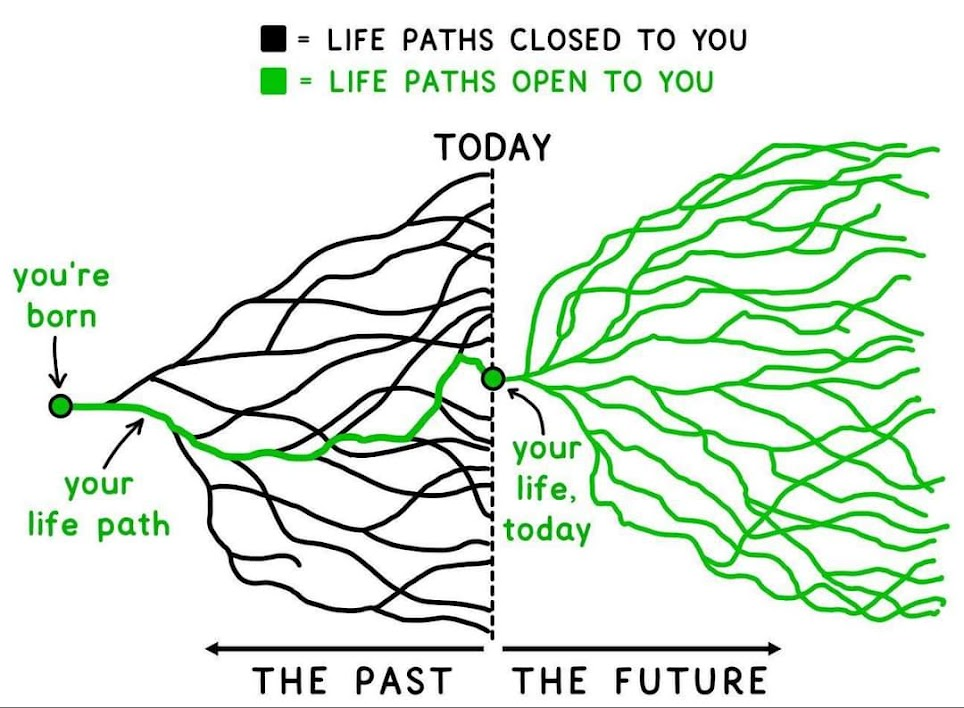
\includegraphics[width=\linewidth]{StochasticTree.jpg}
            \end{figure}
        \end{column}
    \end{columns}
\end{frame}

\begin{frame}{Handling Uncertainty}
    \begin{columns}
        \begin{column}{0.5\textwidth}
            \begin{itemize}
                \item Some variables are shared by all scenarios
                \begin{itemize}
                    \item Decisions that need to be made here and now that impact all scenarios moving forward.
                \end{itemize}
                \item Some variables can be made in the future (and are thus specific to each scenario)
                \begin{itemize}
                    \item Each scenario get's a unique copy of that variable (e.g. iterate over \textbf{S})
                    \item But at certain points in time, certain scenarios are not yet distinguishable. In order to prevent the solution from "anticipating" future changes that are not yet clear, we need "non-anticipativity constraints"
                    \item For each box, select on representative scenario ($s_1$), all other scenarios ($s_2$) should equal that scenario 
                    \item $X_{s_1,t} = X_{s_2,t} \ \ \ \forall s_2 \in \textbf{S}^{BOX}, t \in \textbf{T}^{BOX}$
                \end{itemize}
            \end{itemize}
        \end{column}
        \begin{column}{0.5\textwidth}
            \begin{figure}
                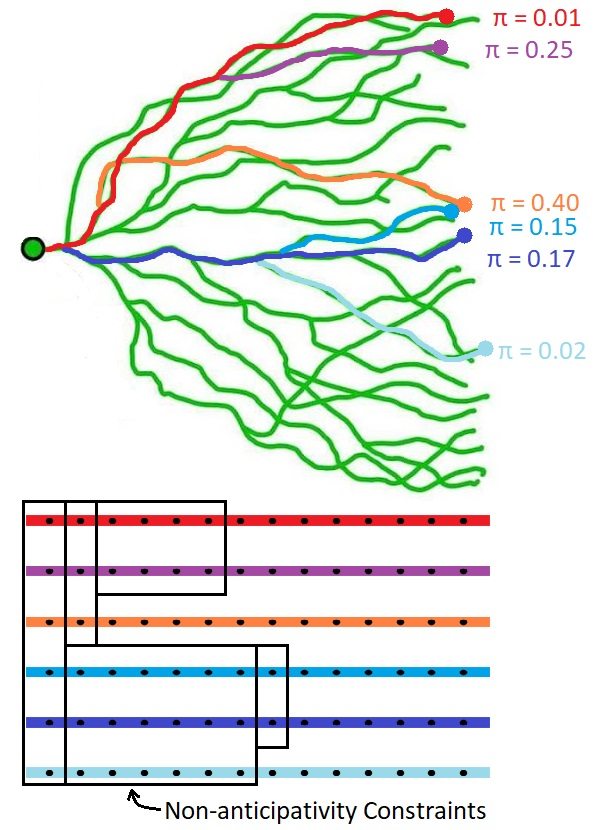
\includegraphics[width=0.75\linewidth]{StochasticTreeHighlight.jpg}
            \end{figure}
        \end{column}
    \end{columns}
\end{frame}

\begin{frame}{Example: Handling Uncertainty}
    \begin{columns}
        \begin{column}{0.5\textwidth}
            \begin{itemize}
                \item Toll rates \textbf{right now} are known.
                \item Toll rates in 1 hour (the next time period) are unknown
                \begin{itemize}
                    \item Congested Scenario ($s_1$)
                    \item Clear roads Scenario ($s_2$)
                \end{itemize}
            \end{itemize}
        \end{column}
        \begin{column}{0.5\textwidth}
            \begin{figure}
                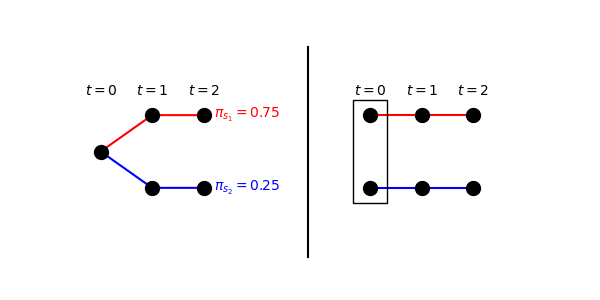
\includegraphics[width=\linewidth]{RoutePlanningProblemWithScenarios.png}
            \end{figure}
        \end{column}
    \end{columns}
    \vspace{-0.7cm}
    \begin{columns}
        \begin{column}{0.4\textwidth}
            \begin{center}
                $\delta_{r,t,s_1}$

                \begin{tabular}{|c||c|c|c|c|}
                    \hline
                    $r$ & $t=0$ & $t=1$ & $t=2$ & $t=3$ \\
                    \hline \hline
                    $AB$ & \$5 & \$10 & \$12 & \$9\\
                    \hline
                    $AC$ & \$30 & \$10 & \$12 & \$ 13\\
                    \hline
                    $BC$ & \$4 & \$5 & \$6 & \$7\\
                    \hline
                    $BD$ & \$2 & \$25 & \$50 & \$2\\
                    \hline
                    $CD$ & \$10 & \$12 & \$13 & \$15\\
                    \hline
                \end{tabular}
            \end{center}
        \end{column}
        \begin{column}{0.4\textwidth}
            \begin{center}
                $\delta_{r,t,s_2}$

                \begin{tabular}{|c||c|c|c|c|}
                    \hline
                    $r$ & $t=0$ & $t=1$ & $t=2$ & $t=3$\\
                    \hline \hline
                    $AB$ & \$5 & \$8 & \$10 & \$7\\
                    \hline
                    $AC$ & \$30 & \$5 & \$9 & \$10\\
                    \hline
                    $BC$ & \$4 & \$10 & \$13 & \$13\\
                    \hline
                    $BD$ & \$2 & \$2 & \$6 & \$6\\
                    \hline
                    $CD$ & \$10 & \$15 & \$4 & \$10\\
                    \hline
                \end{tabular}
            \end{center}
        \end{column}
        \begin{column}{0.2\textwidth}
            \begin{center}
                \begin{tabular}{|c||c|}
                    \hline
                    $s$ & $\pi_s$ \\
                    \hline \hline
                    1 & 0.75 \\
                    \hline
                    2 & 0.25 \\
                    \hline
    
                \end{tabular}
            \end{center}

        \end{column}
    \end{columns}
    \begin{center}
        \textbf{Try on your own (on paper or your computer) to come up with how this problem should be re-formulated.} (5 minutes)
    \end{center}
\end{frame}

\begin{frame}{Example: Handling Uncertainty}
    $$\min_{X_{r,t,s},Y_{r,t,s}} \sum_{s \in \textbf{S}} \pi_s \left( \sum_{r \in \textbf{R}} \sum_{t \in \textbf{T}} \delta_{r,t,s} X_{r,t,s}\right)$$
    $$s.t.\ \ \ Y_{p,t+1,s} - Y_{p,t,s} = \sum_{r\in\textbf{R}^+_p} X_{r,t,s} - \sum_{r\in\textbf{R}^-_p} X_{r,t,s} \ \ \ \forall p \in \textbf{P}, t \in \textbf{T} \neq 3, s \in \textbf{S}$$
    $$\sum_{r \in \textbf{R}} X_{r,t,s} \leq 1 \ \ \ \forall t \in \textbf{T}, s \in \textbf{S}$$
    $$\sum_{p \in \textbf{P}} Y_{p,t,s} = 1 \ \ \ \forall t \in \textbf{T}, s \in \textbf{S}$$
    $$Y_{A,0,s} = 1 \ \ \ \forall s \in \textbf{S}$$
    $$Y_{3,D,s} = 1 \ \ \ \forall s \in \textbf{S}$$
    $$X_{r,0,s_1} = X_{r,0,s} \ \ \ \forall r \in \textbf{R}, s \in \textbf{S} \neq s_1$$
    $$Y_{p,0,s_1} = Y_{p,0,s} \ \ \ \forall p \in \textbf{P}, s \in \textbf{S} \neq s_1$$
    $$X_{r,t,s}, Y_{p,t,s} \in \{0,1\}$$
\end{frame}

\begin{frame}{Linearization}
    \begin{columns}
        \begin{column}{0.5\textwidth}
            \begin{itemize}
                \item Math Modeling only has basic algebra operators: $+,-,\times,\div,\sum,e^x,\log{x},\sin{x},etc.$
                \item Math Modeling does \textbf{not} directly support more advanced operators in the body of a model: $if,then,else,\min(a,b),\max(a,b)$
                \item Remember, problems will solve MUCH faster if we can keep problems as linear as possible.
                \item We can apply some clever tricks to still model these behaviors.
                \item Thought exercise: How can we model the feasible region shown on the right?
            \end{itemize}
        \end{column}
        \begin{column}{0.5\textwidth}
            \begin{figure}
                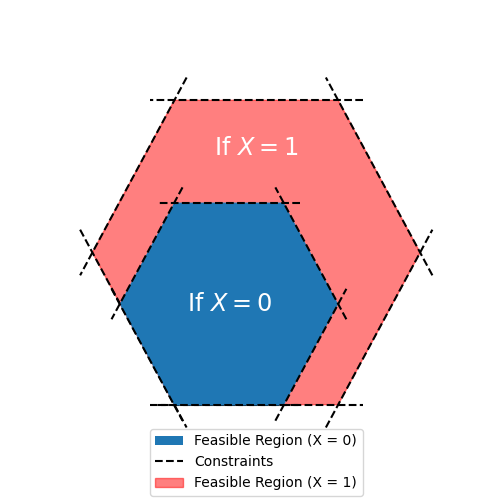
\includegraphics[width=\linewidth]{BigM.png}

            \end{figure}
        \end{column}
    \end{columns}
\end{frame}

\begin{frame}{"Big M" Constraints}
    \vspace{-0.4cm}
    \begin{columns}
        \begin{column}{0.5\textwidth}
            \begin{itemize}
                \item Main Idea: Include an extra term in any constraints that you want to de-activate when a binary variable is 1 (or 0). This extra term should make the constraint so loose that it'll never be binding.
                \item In general, you should just add a binary variable times some \underbar{large} parameter $\mathcal{M}$
                \item Example:
            \end{itemize}
            $$Y \leq 1$$
            $$Y \leq 1 + \mathcal{M} X$$
        \end{column}
        \begin{column}{0.5\textwidth}
            \begin{figure}
                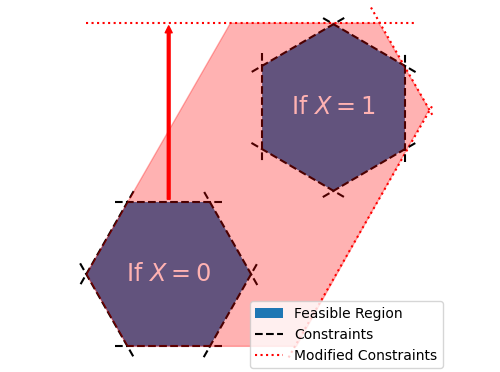
\includegraphics[width=\linewidth]{ExpandedBigM.png}
            \end{figure}
        \end{column}
    \end{columns}
    \begin{itemize}
        \item NOTE OF CAUTION: Choosing a good $\mathcal{M}$ value is the name of the game here:
        \begin{itemize}
            \item Too small: You'll be chopping off parts of the true feasible region. You're problem is likely to become infeasible.
            \item Too big: The solver can get lost and can slow way down.
            \item Too too big: Your computer can't handle huge numbers and (comparatively) tiny numbers at the same time. You're likely to encounter weird errors.
        \end{itemize}
    \end{itemize}
\end{frame}

\begin{frame}{Example: Big M Constraints}
    \begin{columns}
        \begin{column}{0.5\textwidth}
            \begin{itemize}
                \item Let's return to the Route Planning Problem (with Multiple Time Periods, but not Uncertainty)
                \item Let's say there was also an E-Z pass you could purchase for \$12 that gave you a special discount on some, but not all, of the roads in the model.
                \item With the E-Z pass, here would be your $\delta^{EZ}_{r,t}$ values:
            \end{itemize}
            \begin{tabular}{|c||c|c|c|c|}
                \hline
                $r$ & $t=0$ & $t=1$ & $t=2$ & $t=3$ \\
                \hline \hline
                $AB$ & \$0 & \$0 & \$0 & \$0\\
                \hline
                $AC$ & \$5 & \$5 & \$9 & \$10\\
                \hline
                $BC$ & \$4 & \$10 & \$13 & \$13\\
                \hline
                $BD$ & \$2 & \$2 & \$6 & \$5\\
                \hline
                $CD$ & \$0 & \$0 & \$0 & \$0\\
                \hline
            \end{tabular}
        \end{column}
        \begin{column}{0.5\textwidth}
            \begin{figure}
                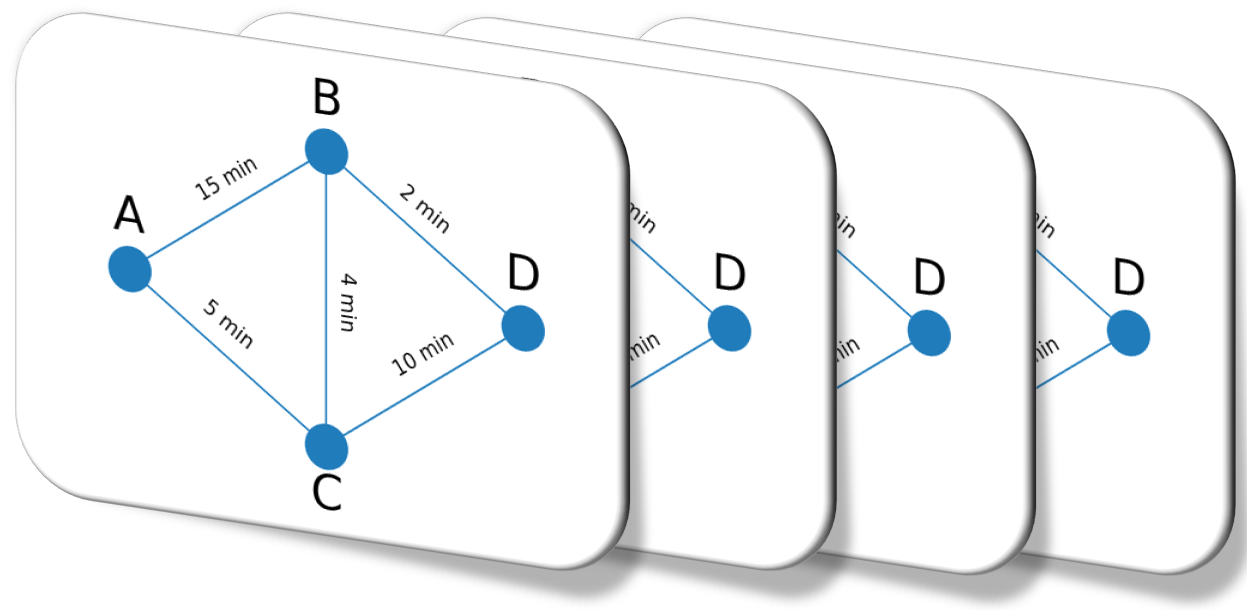
\includegraphics[width=\linewidth]{RoutePlanningProblemRepeated.png}
            \end{figure}
            \begin{itemize}
                \item Should you buy the E-Z pass?
                \item How can you use Big M constraints to capture this decision?
                
                (Spend 5 minutes trying to figure it out)
                \item For the sake of time, we'll move on, but the solution is in the "Solutions.ipynb" notebook on the course website.
            \end{itemize}
        \end{column}
    \end{columns}
\end{frame}

\begin{frame}{"If" Statements}
    \begin{columns}[t]
        \begin{column}[t]{0.5\textwidth}
            \begin{itemize}
                \item Normal "if" statements look like this:
                $$A = \begin{cases}B & if\ X\\C & else \end{cases}$$
                \item We can reformulate this like this:
                $$A = A^B + A^C$$
                $$A^B = \begin{cases}B & if\ X\\0 & else \end{cases} = BX$$
                $$A^C = \begin{cases}C & if\ (1-X)\\0 & else \end{cases} = C(1-X)$$
            \end{itemize}
        \end{column}
        \begin{column}[t]{0.5\textwidth}
            \begin{itemize}
                \item But remember! We want things to be linear!
                \item We can reformulate $A = BX$ using a series of Big M Constraints:
                $$A \leq \beta^{MAX} X$$
                $$A \leq B + \beta^{MIN}(X-1)$$
                $$A \geq \beta^{MIN}X$$
                $$A \geq B + \beta^{MAX}(X-1)$$
                \item Here, $\beta^{MAX}$ and $\beta^{MIN}$ are the maximum and minimum values that $B$ is capable of being. (Big Ms)
                \item If $C$ is not 0, repeat this process for C replacing $X$ with $1-X$.
            \end{itemize}
        \end{column}
    \end{columns}
\end{frame}

\begin{frame}{"If" Statement Caveats}
    \begin{columns}
        \begin{column}{0.5\textwidth}
            \begin{center}
                Explanation of how to come up with the linearization of $A=BX$:
                \begin{figure}
                    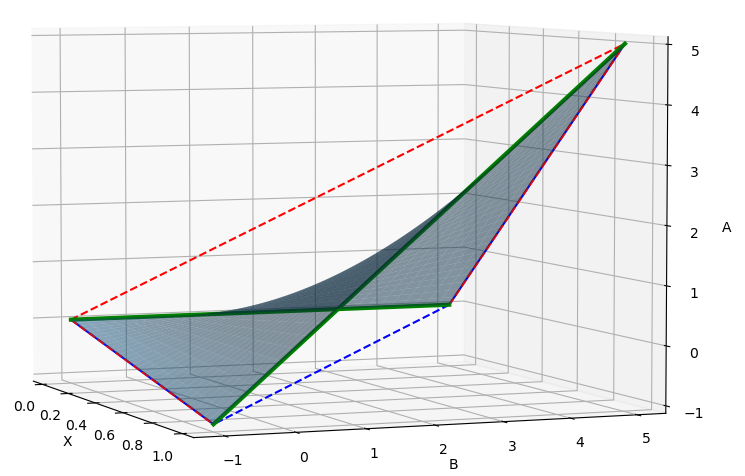
\includegraphics[width=\linewidth]{DoubleSidedBigM.png}
                \end{figure}
            \end{center}
            \begin{tabular}{c c}
                $A \leq \beta^{MAX} X$ & $A \geq \beta^{MIN}X$ \\
                $A \leq B + \beta^{MIN}(X-1)$ & $A \geq B + \beta^{MAX}(X-1)$
            \end{tabular}
        \end{column}
        \begin{column}{0.5\textwidth}

            \begin{itemize}
                \item Sometimes the objective you define indicates that $A$ will always be maximized or minimized.
                \item If you're certain that $A$ will ONLY ever be either maximized or minimized, you can drop two of the constraints.
                \begin{itemize}
                    \item Maximize $A$, drop "Greater Than" Constraints
                    \item Minimize $A$, drop "Less Than" Constraints
                \end{itemize}
                \item Dropping unnecessary constraints means there are less things for the solver to consider: The solver will go faster.
            \end{itemize}
        \end{column}
    \end{columns}
\end{frame}

\begin{frame}[t]{"Max" Statements}
    \begin{center}
        \textbf{IMPORTANT CONSIDERATION: Maximizing or Minimizing $A$}
    \end{center}
    \begin{columns}[t]
        \begin{column}[t]{0.5\textwidth}
            \vspace{-.8cm}
            \begin{center}
                \underbar{If you will allways be minimizing $A=max(B,C)$},
                \underbar{}
            \end{center}
            \vspace{-0.4cm}
            \begin{itemize}
                \item Model this as two individual inequalities (no binary variable needed!):
                $$A \geq B$$
                $$A \geq C$$
            \end{itemize}
            \begin{center}
                \underbar{If you'll be maximizing $A=max(B,C)$}
                \underbar{or you're not sure},
            \end{center}
            \begin{itemize}
                \item You'll need to use a binary variable with and the Big M constraints shown on the right.
            \end{itemize}
        \end{column}
        \begin{column}[t]{0.5\textwidth}
                $$B - C \leq \mathcal{M} Y$$
                $$C - B \leq \mathcal{M} (1-Y)$$
                $$A \geq B$$
                $$A \geq C$$
                $$A \leq B + \mathcal{M}(1-Y)$$
                $$A \leq C + \mathcal{M}Y$$

                Here, $\mathcal{M}$ is the maximum possible difference between $B$ and $C$($\max{\left|B-C\right|}$) and $Y$ is a new binary variable.
        \end{column}
    \end{columns}
\end{frame}

\begin{frame}[t]{"Min" Statements}
    \begin{center}
        \textbf{IMPORTANT CONSIDERATION: Maximizing or Minimizing $A$}
    \end{center}
    \begin{columns}[t]
        \begin{column}[t]{0.5\textwidth}
            \vspace{-.8cm}
            \begin{center}
                \underbar{If you will allways be maximizing $A=min(B,C)$},
                \underbar{}
            \end{center}
            \vspace{-0.4cm}
            \begin{itemize}
                \item Model this as two individual inequalities (no binary variable needed!):
                $$A \leq B$$
                $$A \leq C$$
            \end{itemize}
            \begin{center}
                \underbar{If you'll be minimizing $A=max(B,C)$}
                \underbar{or you're not sure},
            \end{center}
            \begin{itemize}
                \item You'll need to use a binary variable with and the Big M constraints shown on the right.
            \end{itemize}
        \end{column}
        \begin{column}[t]{0.5\textwidth}
                $$C - B \leq \mathcal{M} Y$$
                $$B - C \leq \mathcal{M} (1-Y)$$
                $$A \leq B$$
                $$A \leq C$$
                $$A \geq B - \mathcal{M}(1-Y)$$
                $$A \geq C - \mathcal{M}Y$$

                Here, $\mathcal{M}$ is the maximum possible difference between $B$ and $C$($\max{\left|B-C\right|}$) and $Y$ is a new binary variable.
        \end{column}
    \end{columns}
\end{frame}

\begin{frame}{Next Class: Real life Problems}
    \begin{itemize}
        \item Now that we have some powerful tools to capture real-world behaviors, we can jump into some real-world problems.
        \item I'd love to go over some problems you might be thinking of.
        \begin{itemize}
            \item Do you have any requests?
        \end{itemize}
        \item Problems I've already considered are:
        \begin{itemize}
            \item How can I most effectively schedule tasks in my daily schedule?
            \item How can I make a good choice about which insurance plan to select?
            \item What's the most efficient way to transfer money between my bank accounts to pay my bills?
        \end{itemize}
    \end{itemize}
\end{frame}

\end{document}